% Options for packages loaded elsewhere
\PassOptionsToPackage{unicode}{hyperref}
\PassOptionsToPackage{hyphens}{url}
%
\documentclass[
]{book}
\usepackage{amsmath,amssymb}
\usepackage{lmodern}
\usepackage{ifxetex,ifluatex}
\ifnum 0\ifxetex 1\fi\ifluatex 1\fi=0 % if pdftex
  \usepackage[T1]{fontenc}
  \usepackage[utf8]{inputenc}
  \usepackage{textcomp} % provide euro and other symbols
\else % if luatex or xetex
  \usepackage{unicode-math}
  \defaultfontfeatures{Scale=MatchLowercase}
  \defaultfontfeatures[\rmfamily]{Ligatures=TeX,Scale=1}
\fi
% Use upquote if available, for straight quotes in verbatim environments
\IfFileExists{upquote.sty}{\usepackage{upquote}}{}
\IfFileExists{microtype.sty}{% use microtype if available
  \usepackage[]{microtype}
  \UseMicrotypeSet[protrusion]{basicmath} % disable protrusion for tt fonts
}{}
\makeatletter
\@ifundefined{KOMAClassName}{% if non-KOMA class
  \IfFileExists{parskip.sty}{%
    \usepackage{parskip}
  }{% else
    \setlength{\parindent}{0pt}
    \setlength{\parskip}{6pt plus 2pt minus 1pt}}
}{% if KOMA class
  \KOMAoptions{parskip=half}}
\makeatother
\usepackage{xcolor}
\IfFileExists{xurl.sty}{\usepackage{xurl}}{} % add URL line breaks if available
\IfFileExists{bookmark.sty}{\usepackage{bookmark}}{\usepackage{hyperref}}
\hypersetup{
  pdftitle={EVALUACION DE TIERRAS},
  pdfauthor={Profesores Victor Sevilla, Juan Carlos Rey y Barbara Rodriguez},
  hidelinks,
  pdfcreator={LaTeX via pandoc}}
\urlstyle{same} % disable monospaced font for URLs
\usepackage{color}
\usepackage{fancyvrb}
\newcommand{\VerbBar}{|}
\newcommand{\VERB}{\Verb[commandchars=\\\{\}]}
\DefineVerbatimEnvironment{Highlighting}{Verbatim}{commandchars=\\\{\}}
% Add ',fontsize=\small' for more characters per line
\usepackage{framed}
\definecolor{shadecolor}{RGB}{248,248,248}
\newenvironment{Shaded}{\begin{snugshade}}{\end{snugshade}}
\newcommand{\AlertTok}[1]{\textcolor[rgb]{0.94,0.16,0.16}{#1}}
\newcommand{\AnnotationTok}[1]{\textcolor[rgb]{0.56,0.35,0.01}{\textbf{\textit{#1}}}}
\newcommand{\AttributeTok}[1]{\textcolor[rgb]{0.77,0.63,0.00}{#1}}
\newcommand{\BaseNTok}[1]{\textcolor[rgb]{0.00,0.00,0.81}{#1}}
\newcommand{\BuiltInTok}[1]{#1}
\newcommand{\CharTok}[1]{\textcolor[rgb]{0.31,0.60,0.02}{#1}}
\newcommand{\CommentTok}[1]{\textcolor[rgb]{0.56,0.35,0.01}{\textit{#1}}}
\newcommand{\CommentVarTok}[1]{\textcolor[rgb]{0.56,0.35,0.01}{\textbf{\textit{#1}}}}
\newcommand{\ConstantTok}[1]{\textcolor[rgb]{0.00,0.00,0.00}{#1}}
\newcommand{\ControlFlowTok}[1]{\textcolor[rgb]{0.13,0.29,0.53}{\textbf{#1}}}
\newcommand{\DataTypeTok}[1]{\textcolor[rgb]{0.13,0.29,0.53}{#1}}
\newcommand{\DecValTok}[1]{\textcolor[rgb]{0.00,0.00,0.81}{#1}}
\newcommand{\DocumentationTok}[1]{\textcolor[rgb]{0.56,0.35,0.01}{\textbf{\textit{#1}}}}
\newcommand{\ErrorTok}[1]{\textcolor[rgb]{0.64,0.00,0.00}{\textbf{#1}}}
\newcommand{\ExtensionTok}[1]{#1}
\newcommand{\FloatTok}[1]{\textcolor[rgb]{0.00,0.00,0.81}{#1}}
\newcommand{\FunctionTok}[1]{\textcolor[rgb]{0.00,0.00,0.00}{#1}}
\newcommand{\ImportTok}[1]{#1}
\newcommand{\InformationTok}[1]{\textcolor[rgb]{0.56,0.35,0.01}{\textbf{\textit{#1}}}}
\newcommand{\KeywordTok}[1]{\textcolor[rgb]{0.13,0.29,0.53}{\textbf{#1}}}
\newcommand{\NormalTok}[1]{#1}
\newcommand{\OperatorTok}[1]{\textcolor[rgb]{0.81,0.36,0.00}{\textbf{#1}}}
\newcommand{\OtherTok}[1]{\textcolor[rgb]{0.56,0.35,0.01}{#1}}
\newcommand{\PreprocessorTok}[1]{\textcolor[rgb]{0.56,0.35,0.01}{\textit{#1}}}
\newcommand{\RegionMarkerTok}[1]{#1}
\newcommand{\SpecialCharTok}[1]{\textcolor[rgb]{0.00,0.00,0.00}{#1}}
\newcommand{\SpecialStringTok}[1]{\textcolor[rgb]{0.31,0.60,0.02}{#1}}
\newcommand{\StringTok}[1]{\textcolor[rgb]{0.31,0.60,0.02}{#1}}
\newcommand{\VariableTok}[1]{\textcolor[rgb]{0.00,0.00,0.00}{#1}}
\newcommand{\VerbatimStringTok}[1]{\textcolor[rgb]{0.31,0.60,0.02}{#1}}
\newcommand{\WarningTok}[1]{\textcolor[rgb]{0.56,0.35,0.01}{\textbf{\textit{#1}}}}
\usepackage{longtable,booktabs,array}
\usepackage{calc} % for calculating minipage widths
% Correct order of tables after \paragraph or \subparagraph
\usepackage{etoolbox}
\makeatletter
\patchcmd\longtable{\par}{\if@noskipsec\mbox{}\fi\par}{}{}
\makeatother
% Allow footnotes in longtable head/foot
\IfFileExists{footnotehyper.sty}{\usepackage{footnotehyper}}{\usepackage{footnote}}
\makesavenoteenv{longtable}
\usepackage{graphicx}
\makeatletter
\def\maxwidth{\ifdim\Gin@nat@width>\linewidth\linewidth\else\Gin@nat@width\fi}
\def\maxheight{\ifdim\Gin@nat@height>\textheight\textheight\else\Gin@nat@height\fi}
\makeatother
% Scale images if necessary, so that they will not overflow the page
% margins by default, and it is still possible to overwrite the defaults
% using explicit options in \includegraphics[width, height, ...]{}
\setkeys{Gin}{width=\maxwidth,height=\maxheight,keepaspectratio}
% Set default figure placement to htbp
\makeatletter
\def\fps@figure{htbp}
\makeatother
\setlength{\emergencystretch}{3em} % prevent overfull lines
\providecommand{\tightlist}{%
  \setlength{\itemsep}{0pt}\setlength{\parskip}{0pt}}
\setcounter{secnumdepth}{5}
\usepackage{booktabs}
\ifluatex
  \usepackage{selnolig}  % disable illegal ligatures
\fi
\usepackage[]{natbib}
\bibliographystyle{plainnat}

\title{EVALUACION DE TIERRAS}
\author{Profesores Victor Sevilla, Juan Carlos Rey y Barbara Rodriguez}
\date{2022-09-30}

\begin{document}
\maketitle

{
\setcounter{tocdepth}{1}
\tableofcontents
}
\hypertarget{introduccion-a-la-asignatura}{%
\chapter{Introduccion a la asignatura}\label{introduccion-a-la-asignatura}}

\begin{center}\rule{0.5\linewidth}{0.5pt}\end{center}

\hypertarget{bienvenida}{%
\section*{Bienvenida}\label{bienvenida}}
\addcontentsline{toc}{section}{Bienvenida}

Bienvenidos a la Asignatura \textbf{Evaluacion de Tierras}. Cada uno de los iconos ubicados abajo son enlaces hacia información sobre la materia, como: objetivos, normas de la cátedra, programa de la asignatura, entre otros. Le sugerimos que comiences por leer las \emph{Instrucciones} y luego podra navegar libremente por todas las secciones.

\begin{center}\rule{0.5\linewidth}{0.5pt}\end{center}

\hypertarget{instrucciones}{%
\section*{Instrucciones}\label{instrucciones}}
\addcontentsline{toc}{section}{Instrucciones}

En esta página encontrará diferentes elementos necesarios para cursar con éxito nuestra asignatura, tales como: indicaciones generales, programación de actividades, sistemas de evaluación, entre muchas más información. Además podrá descargar las presentaciones teóricas y guías prácticas en formatos documentos, datos para el trabajo extra - aula, inclusives encontrará enlaces que lo llevaran a los videos y formularios disponibles en la asignatura.

Puede seguir los enlaces disponibles dentro del texto para moverse entre diferentes elementos y aspectos que comprende esta página.

Esta página ha sido diseñada para complementar las actividades presenciales (sesiones teóricas y prácticas) y para tratar de maximizar las interacciones entre alumnos y profesores sobre las actividades a realizar.

También en esta página podrá revisar las calificaciones, lo que te permitirá llevar un registro de tu rendimiento académico.

\begin{center}\rule{0.5\linewidth}{0.5pt}\end{center}

\hypertarget{objetivos}{%
\section*{Objetivos}\label{objetivos}}
\addcontentsline{toc}{section}{Objetivos}

\hypertarget{general}{%
\subsubsection*{General}\label{general}}
\addcontentsline{toc}{subsubsection}{General}

El objetivo general de esta asignatura es capacitar a los estudiantes en la evaluación e interpretación de información básica sobre clima, biota, hidrología, suelos, geología y geomorfología, para establecer la capacidad de uso agropecuario que posean las tierras y su aptitud para usos agrícolas específicos sostenibles.

\hypertarget{especuxedficos}{%
\subsubsection*{Específicos}\label{especuxedficos}}
\addcontentsline{toc}{subsubsection}{Específicos}

\begin{itemize}
\tightlist
\item
  Repasar conceptos generales de Clasificación taxonómica y Cartografía de los suelos.
\item
  Conocer la variabilidad espacial de las tierras en el país, evidenciando limitaciones, potencialidades y suelos de referencia.
\item
  Aplicar los fundamentos de la Evaluación de las Tierras, mediante las metodologías empleadas en el país altamente comprobadas y de uso generalizado.
\item
  Evaluar en campo las tierras en parcelas agropecuarias con limitada información.
\end{itemize}

\begin{center}\rule{0.5\linewidth}{0.5pt}\end{center}

\hypertarget{normas}{%
\section*{Normas}\label{normas}}
\addcontentsline{toc}{section}{Normas}

Evaluación de Tierras es una asignatura del séptimo semestre, y se dicta en una sesión Teórica-práctica de 3 horas de duración los días jueves y viernes en el horario de 1:30 pm -- 4:45 pm en aulas del Departamento de Edafología.

Las sesiones Teórico-prácticas son de obligatoria asistencia, tal como lo establece el reglamento vigente.

Debes asistir a la sección Teórico-prácticas en la cual se inscribió; no puedes recuperar prácticas en otro grupo sin la debida autorización de su profesor y del profesor del grupo al cual quieres asistir.

Solo se te permitirá la recuperación de una práctica por cada Unidad de la asignatura.

La no asistencia o incumplimiento de las actividades programadas por la Cátedra deberá ser informada por escrito a la Cátedra dentro de las 48 horas de haber ocurrido la falta, incluyendo las constancias y los avales necesarios para su justificación.

Deberás entregar la comunicación y los avales respectivos en la Secretaría del Departamento de Edafología o enviarla al correo electrónico del profesor \href{mailto:samoy315@gmail.com}{\nolinkurl{samoy315@gmail.com}}, donde será considerada en la próxima reunión de cátedra.

Si tienes algún problema personal o actividad permanente que le impida asistir a las clases, debes dirigirte a la Dirección de Escuela o al Consejo de Facultad solicitando aval para las inasistencias, pues la Cátedra no tiene potestad para hacerlo.

La cátedra de Evaluación de Tierras, con sus profesores y todo el personal de apoyo, están a su disposición para orientarte y ayudarte a solventar los problemas que se le puedan presentar, siempre y cuando acudas a ellos, conozcan y acaten las reglas establecidas y asuma con responsabilidad el compromiso con la asignatura.

\begin{center}\rule{0.5\linewidth}{0.5pt}\end{center}

\hypertarget{como-aprobar}{%
\section*{¿Como aprobar?}\label{como-aprobar}}
\addcontentsline{toc}{section}{¿Como aprobar?}

Para poder aprobar esta asignatura, deberá obtener una calificación mínima acumulada de 10 puntos (escala de 1 al 20 puntos), basado en la información que se presenta en el siguiente cuadro 1. Las evaluaciones perdidas contarán como cero puntos.

\emph{Cuadro 1. Plan de evaluacion de la asignatura}

\begin{longtable}[]{@{}
  >{\centering\arraybackslash}p{(\columnwidth - 4\tabcolsep) * \real{0.33}}
  >{\centering\arraybackslash}p{(\columnwidth - 4\tabcolsep) * \real{0.33}}
  >{\centering\arraybackslash}p{(\columnwidth - 4\tabcolsep) * \real{0.33}}@{}}
\toprule
Unidades & Actividades & Ponderacion \\
\midrule
\endhead
1.Variabilidad de las tierras en Venezuela & Asignacion (tareas) y Prueba cortas & 30\% \\
1 & 2 & 3 \\
1 & 2 & 3 \\
\bottomrule
\end{longtable}

\begin{center}\rule{0.5\linewidth}{0.5pt}\end{center}

\hypertarget{profesores}{%
\section*{Profesores}\label{profesores}}
\addcontentsline{toc}{section}{Profesores}

\emph{Cuadro 2. Profesores de la asignatura \textbf{Evaluacion de Tierras}}

\href{https://github.com/JoseCaicedoDev/cardReact/files/9688200/rmarkdown_reference.pdf}{rmarkdown\_reference.pdf}

Aqui podra descargar el libro de Hobbit \href{pdf/hobbit.pdf}{Libro del Hobbit}

\hypertarget{teorias}{%
\chapter{Teorias}\label{teorias}}

All chapters start with a first-level heading followed by your chapter title, like the line above. There should be only one first-level heading (\texttt{\#}) per .Rmd file.

\hypertarget{a-section}{%
\section{A section}\label{a-section}}

All chapter sections start with a second-level (\texttt{\#\#}) or higher heading followed by your section title, like the sections above and below here. You can have as many as you want within a chapter.

\hypertarget{an-unnumbered-section}{%
\subsection*{An unnumbered section}\label{an-unnumbered-section}}
\addcontentsline{toc}{subsection}{An unnumbered section}

Chapters and sections are numbered by default. To un-number a heading, add a \texttt{\{.unnumbered\}} or the shorter \texttt{\{-\}} at the end of the heading, like in this section.

\hypertarget{cross}{%
\chapter{Practicas}\label{cross}}

Cross-references make it easier for your readers to find and link to elements in your book.

There are two steps to cross-reference any heading:

\begin{enumerate}
\def\labelenumi{\arabic{enumi}.}
\tightlist
\item
  Label the heading: \texttt{\#\ Hello\ world\ \{\#nice-label\}}.

  \begin{itemize}
  \tightlist
  \item
    Leave the label off if you like the automated heading generated based on your heading title: for example, \texttt{\#\ Hello\ world} = \texttt{\#\ Hello\ world\ \{\#hello-world\}}.
  \item
    To label an un-numbered heading, use: \texttt{\#\ Hello\ world\ \{-\#nice-label\}} or \texttt{\{\#\ Hello\ world\ .unnumbered\}}.
  \end{itemize}
\item
  Next, reference the labeled heading anywhere in the text using \texttt{\textbackslash{}@ref(nice-label)}; for example, please see Chapter \ref{cross}.

  \begin{itemize}
  \tightlist
  \item
    If you prefer text as the link instead of a numbered reference use: \protect\hyperlink{cross}{any text you want can go here}.
  \end{itemize}
\end{enumerate}

\hypertarget{unidad-1}{%
\section*{Unidad 1}\label{unidad-1}}
\addcontentsline{toc}{section}{Unidad 1}

\hypertarget{semana-0}{%
\subsection*{Semana 0}\label{semana-0}}
\addcontentsline{toc}{subsection}{Semana 0}

\hypertarget{semana-1}{%
\subsection*{Semana 1}\label{semana-1}}
\addcontentsline{toc}{subsection}{Semana 1}

\hypertarget{taxonomia-de-los-suelos}{%
\subsubsection*{Taxonomia de los Suelos}\label{taxonomia-de-los-suelos}}
\addcontentsline{toc}{subsubsection}{Taxonomia de los Suelos}

\hypertarget{semana-2}{%
\subsection*{Semana 2}\label{semana-2}}
\addcontentsline{toc}{subsection}{Semana 2}

\hypertarget{semana-3}{%
\subsection*{Semana 3}\label{semana-3}}
\addcontentsline{toc}{subsection}{Semana 3}

\hypertarget{semana-4}{%
\subsection*{Semana 4}\label{semana-4}}
\addcontentsline{toc}{subsection}{Semana 4}

Figures and tables \emph{with captions} can also be cross-referenced from elsewhere in your book using \texttt{\textbackslash{}@ref(fig:chunk-label)} and \texttt{\textbackslash{}@ref(tab:chunk-label)}, respectively.

See Figure \ref{fig:nice-fig}.

\begin{Shaded}
\begin{Highlighting}[]
\FunctionTok{par}\NormalTok{(}\AttributeTok{mar =} \FunctionTok{c}\NormalTok{(}\DecValTok{4}\NormalTok{, }\DecValTok{4}\NormalTok{, .}\DecValTok{1}\NormalTok{, .}\DecValTok{1}\NormalTok{))}
\FunctionTok{plot}\NormalTok{(pressure, }\AttributeTok{type =} \StringTok{\textquotesingle{}b\textquotesingle{}}\NormalTok{, }\AttributeTok{pch =} \DecValTok{19}\NormalTok{)}
\end{Highlighting}
\end{Shaded}

\begin{figure}

{\centering 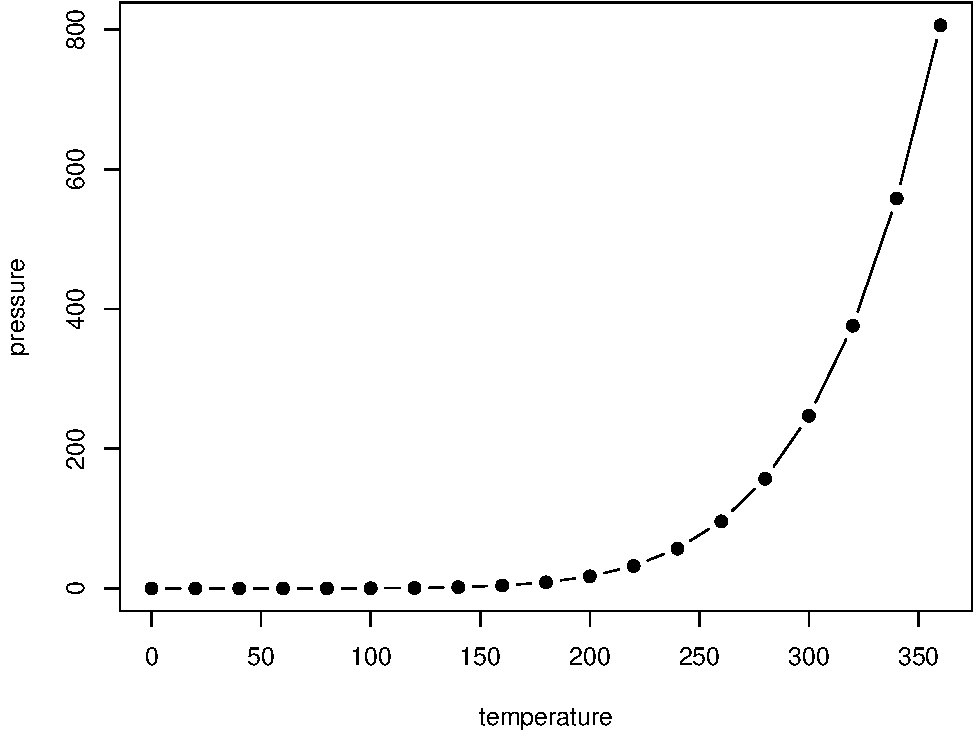
\includegraphics[width=0.8\linewidth]{_main_files/figure-latex/nice-fig-1} 

}

\caption{Here is a nice figure!}\label{fig:nice-fig}
\end{figure}

Don't miss Table \ref{tab:nice-tab}.

\begin{Shaded}
\begin{Highlighting}[]
\NormalTok{knitr}\SpecialCharTok{::}\FunctionTok{kable}\NormalTok{(}
  \FunctionTok{head}\NormalTok{(pressure, }\DecValTok{10}\NormalTok{), }\AttributeTok{caption =} \StringTok{\textquotesingle{}Here is a nice table!\textquotesingle{}}\NormalTok{,}
  \AttributeTok{booktabs =} \ConstantTok{TRUE}
\NormalTok{)}
\end{Highlighting}
\end{Shaded}

\begin{table}

\caption{\label{tab:nice-tab}Here is a nice table!}
\centering
\begin{tabular}[t]{rr}
\toprule
temperature & pressure\\
\midrule
0 & 0.0002\\
20 & 0.0012\\
40 & 0.0060\\
60 & 0.0300\\
80 & 0.0900\\
\addlinespace
100 & 0.2700\\
120 & 0.7500\\
140 & 1.8500\\
160 & 4.2000\\
180 & 8.8000\\
\bottomrule
\end{tabular}
\end{table}

\hypertarget{unidad-2}{%
\section*{Unidad 2}\label{unidad-2}}
\addcontentsline{toc}{section}{Unidad 2}

\hypertarget{semana-5}{%
\subsection*{Semana 5}\label{semana-5}}
\addcontentsline{toc}{subsection}{Semana 5}

\hypertarget{semana-6}{%
\subsection*{Semana 6}\label{semana-6}}
\addcontentsline{toc}{subsection}{Semana 6}

\hypertarget{semana-7}{%
\subsection*{Semana 7}\label{semana-7}}
\addcontentsline{toc}{subsection}{Semana 7}

\hypertarget{semana-8}{%
\subsection*{Semana 8}\label{semana-8}}
\addcontentsline{toc}{subsection}{Semana 8}

\hypertarget{semana-9}{%
\subsection*{Semana 9}\label{semana-9}}
\addcontentsline{toc}{subsection}{Semana 9}

\hypertarget{semana-10}{%
\subsection*{Semana 10}\label{semana-10}}
\addcontentsline{toc}{subsection}{Semana 10}

\hypertarget{unidad-3}{%
\section*{Unidad 3}\label{unidad-3}}
\addcontentsline{toc}{section}{Unidad 3}

\hypertarget{semana-11}{%
\subsection*{Semana 11}\label{semana-11}}
\addcontentsline{toc}{subsection}{Semana 11}

\hypertarget{semana-12}{%
\subsection*{Semana 12}\label{semana-12}}
\addcontentsline{toc}{subsection}{Semana 12}

\hypertarget{semana-13}{%
\subsection*{Semana 13}\label{semana-13}}
\addcontentsline{toc}{subsection}{Semana 13}

\hypertarget{semana-14}{%
\subsection*{Semana 14}\label{semana-14}}
\addcontentsline{toc}{subsection}{Semana 14}

\hypertarget{semana-15}{%
\subsection*{Semana 15}\label{semana-15}}
\addcontentsline{toc}{subsection}{Semana 15}

\hypertarget{trabajo-extra---aula}{%
\chapter{Trabajo Extra - aula}\label{trabajo-extra---aula}}

You can add parts to organize one or more book chapters together. Parts can be inserted at the top of an .Rmd file, before the first-level chapter heading in that same file.

Add a numbered part: \texttt{\#\ (PART)\ Act\ one\ \{-\}} (followed by \texttt{\#\ A\ chapter})

Add an unnumbered part: \texttt{\#\ (PART\textbackslash{}*)\ Act\ one\ \{-\}} (followed by \texttt{\#\ A\ chapter})

Add an appendix as a special kind of un-numbered part: \texttt{\#\ (APPENDIX)\ Other\ stuff\ \{-\}} (followed by \texttt{\#\ A\ chapter}). Chapters in an appendix are prepended with letters instead of numbers.

\hypertarget{informacion-general}{%
\chapter{Informacion General}\label{informacion-general}}

\hypertarget{estudiantes-2022}{%
\section{Estudiantes 2022}\label{estudiantes-2022}}

\textbf{Cuadro 3. Estudiantes del año 2022}

\begin{longtable}[]{@{}ccc@{}}
\toprule
Estudiantes & Seccion & Grupo \\
\midrule
\endhead
Victor Sevilla & Viernes pm & 2 \\
\bottomrule
\end{longtable}

\hypertarget{citations}{%
\section{Citations}\label{citations}}

Reference items in your bibliography file(s) using \texttt{@key}.

For example, we are using the \textbf{bookdown} package \citep{R-bookdown} (check out the last code chunk in index.Rmd to see how this citation key was added) in this sample book, which was built on top of R Markdown and \textbf{knitr} \citep{xie2015} (this citation was added manually in an external file book.bib).
Note that the \texttt{.bib} files need to be listed in the index.Rmd with the YAML \texttt{bibliography} key.

The RStudio Visual Markdown Editor can also make it easier to insert citations: \url{https://rstudio.github.io/visual-markdown-editing/\#/citations}

  \bibliography{book.bib,packages.bib}

\end{document}
